% Modèles de vision off-the-shelf : outils libres pour l'extraction d’objets

\subsection{YOLOv5, \docex et autres modèles}
    \subsubsection{Utilisation d'un modèle pré-entraîné}
	Il est courant, pour la vision artificielle, d'utiliser un modèle pré-entraîné sur un grand jeu de données peu spécifique, et de l'affiner à partir d'un plus petit jeu de données correspondant précisément aux attentes et applications du modèle dans le projet\footnote{Nous nous focaliserons spécifiquement sur les modèles de détection et de classification, dont la question de l'entraînement a été abordée lors du stage.}. En effet, un modèle entraîné sur un jeu de données de base suffisamment large et généraliste apprend des caractéristiques qui peuvent être appliquées à l'ensemble du monde visuel, et peut ainsi servir de modèle générique pour de nombreux problèmes de vision par ordinateur\footcite{cholletApprentissageProfondAvec2020a}, même si ces derniers sont éloignés de la tâche initiale. La portabilité des caractéristiques apprises rend ainsi l'usage du \dl pertinent dans le cadre de projets de recherche sur des sources historiques, puisqu'elle assure ainsi l'efficacité des modèles créés malgré les possibles limites des jeux de données disponibles : il est ainsi possible d'entraîner un modèle sur un jeu de données limité, qui correspond à la réalité matérielle des sources étudiées. 
	
	\subsubsection{ImageNet} 
	ImageNet\footcite{ImageNet} est une initiative ayant pour objectif de fournir en accès libre un vaste jeu de données images pour la recherche en vision artificielle. Cette initiative est née du besoin crucial de données d'entraînement et de validation pour le \ml, et particulièrement pour la classification, tâche de base de la vision par ordinateur, qui requiert un volume important d'images pour l'obtention de bonnes performances. Le jeu de données ImageNet compte plus d'un million d'images, catégorisées selon des concepts récupérés du projet WordNet qui vise à répertorier et classifier le contenu sémantique et lexical de la langue anglaise. Chaque image du jeu de données est annotée manuellement pour indiquer les objets présent dans l'image : ImageNet est un projet participatif, ce qui permet d'assurer la continuité de son enrichissement. Le projet ne possède pas les droits des images du jeu de données, formulant simplement une liste d'images disponibles sur le Web pour chaque concept WordNet : elles sont mises à disposition des projets à visée non-commerciale, pour assurer aux chercheurs la possibilité de mener des recherches en ayant accès à un jeu de données d'entraînement riche et vaste, permettant de développer des modèles performants avant un entraînement plus spécialisé.
    
    \subsubsection{\yolov : un modèle de pointe pour l'extraction d'objets}
	\yolov\footcite{ultralyticsUltralyticsYOLOv8Docs} est la cinquième version du modèle de détection d'objet et de segmentation d'images \yolo, développé à l'Université de Washington Joseph Redmon et Ali Farhadi et lancé en 2015. \yolov, publié en 2020, est un modèle réputé pour sa rapidité d'exécution et sa précision\footcite{buttnerCorDeepSacroboscoDataset2022}, pré-entraîné sur le jeu de données MS COCO\footcite{COCOCommonObjects}, dont l'implémentation se veut aisée : \yolov, contrairement à ses prédécesseurs, est directement implémenté dans PyTorch\footcite{PyTorch}, permettant une intégration facile à un environnement de développement, puisqu'il nécessite moins d'adaptation que les versions précédentes fonctionnant avec le \textit{framework} Darknet\footcite{DarknetOpenSource}, basé sur le langage C\footcite{sharmaTrainingYOLOv5Object2022}. Le réseau neuronal de \yolo fonctionne en trois étapes : l'extraction de caractéristiques des données d'entrée, l'agrégation de ces caractéristiques, puis la résolution du problème (dans ce cas précis, la détection des objets)\footcite{buttnerCorDeepSacroboscoDataset2022} Le modèle est disponible en accès libre, et constitue ainsi une base solide pour les projets souhaitant utiliser un modèle de détection d'objet : \yolov peut, en effet, être entraîné sur un jeu de données choisi, pour en affiner la détection et l'appliquer à des images plus spécifiques, telles que des pages d'ouvrages.
	
	Les projets \eida et \vhs entraînent, pour la détection d'illustrations dans les numérisations d'ouvrages, des modèles ayant pour base \yolov. Sans entraînement spécifique, en s'appuyant exclusivement sur le pré-entraînement fait avant la mise en ligne du modèle, les performances sont peu satisfaisantes : les jeux de données utilisés pour ce pré-entraînement, qu'il s'agisse d'ImageNet ou de MS COCO, sont en effet des jeux de données d'images réelles, faits pour l'apprentissage de la classification d'objets du quotidien, et ne sont donc initialement pas adaptés à la segmentation de pages de manuscrits ou à la détection d'illustrations. Il faut ainsi compter sur les propriétés de portabilité de l'apprentissage, qui assurent que ce pré-entraînement sur des images réelles permet d'accélérer le processus de développement du modèle, puisqu'elles permettent de s'intéresser immédiatement à l'entraînement à partir de données spécifiques, et réduisent le volume nécessaire. 
	
	\subsubsection{\docex : un modèle pour les sources historiques}
   	\docex est un modèle \textit{off-the-shelf} de détection d'objet, dédié spécifiquement aux documents historiques\footcite{monnierDocExtractorOfftheshelfHistorical2020}. Développé par Tom Monnier, ce modèle a pour vocation d'être un outil efficace et prêt à l'usage pour le traitement de documents numérisés, capable de détecter le texte et segmenter les lignes, et d'extraire les illustrations en détectant leurs contours précis\footnote{Contrairement à \yolov qui produit des annotations rectangulaires et ne gère pas les polygones.}. \docex est entraîné à partir d'images produites par un générateur de documents historiques synthétiques (fig. \ref{fig:syndoc}), qui promet de bonnes performances même sans \textit{fine-tuning} : l'utilisation de ce générateur automatique, appelé SynDoc\footnote{Les images générées par SynDoc sont composées aléatoirement à partir d'une sélection d'images de fonds (pages et contextes), auxquelles sont ajoutées une mise en page selon laquelle est disposé un contenu image et texte, puis du bruit. Tous ces éléments sont tirés d'un jeu d'images pré-établi (constitué de 177 images de pages, 15 contextes, plus de 8000 œuvres d'art provenant de WikiArt, des lettrines générées à partir d'une lettre aléatoire avec 91 fonts possibles, et des dessins, schémas et textes tirés d'articles aléatoires sur Wikipedia, avec plus de 400 fonts) et composent des pages aléatoires mêlant images, texte et bruit, avec un nombre vaste de possibilités qui égale les plus grands jeu de données d'entraînement. Ces pages ne nécessitent pas d'annotations manuelles, puisque chaque élément de contenu est pré-annoté.}, vise à répondre aux problématiques de création de jeux de données d'entraînement à partir de documents historiques, limités à la fois par le nombre de documents disponibles et les moyens humains que l'annotation d'images nécessite. SynDoc permet ainsi, dans la création d'un modèle, de combler l'absence d'un jeu de données de grande échelle d'images de documents historiques annotées\footcite{buttnerCorDeepSacroboscoDataset2022}.
   	
   	\begin{figure}[h]
   		\centering
   		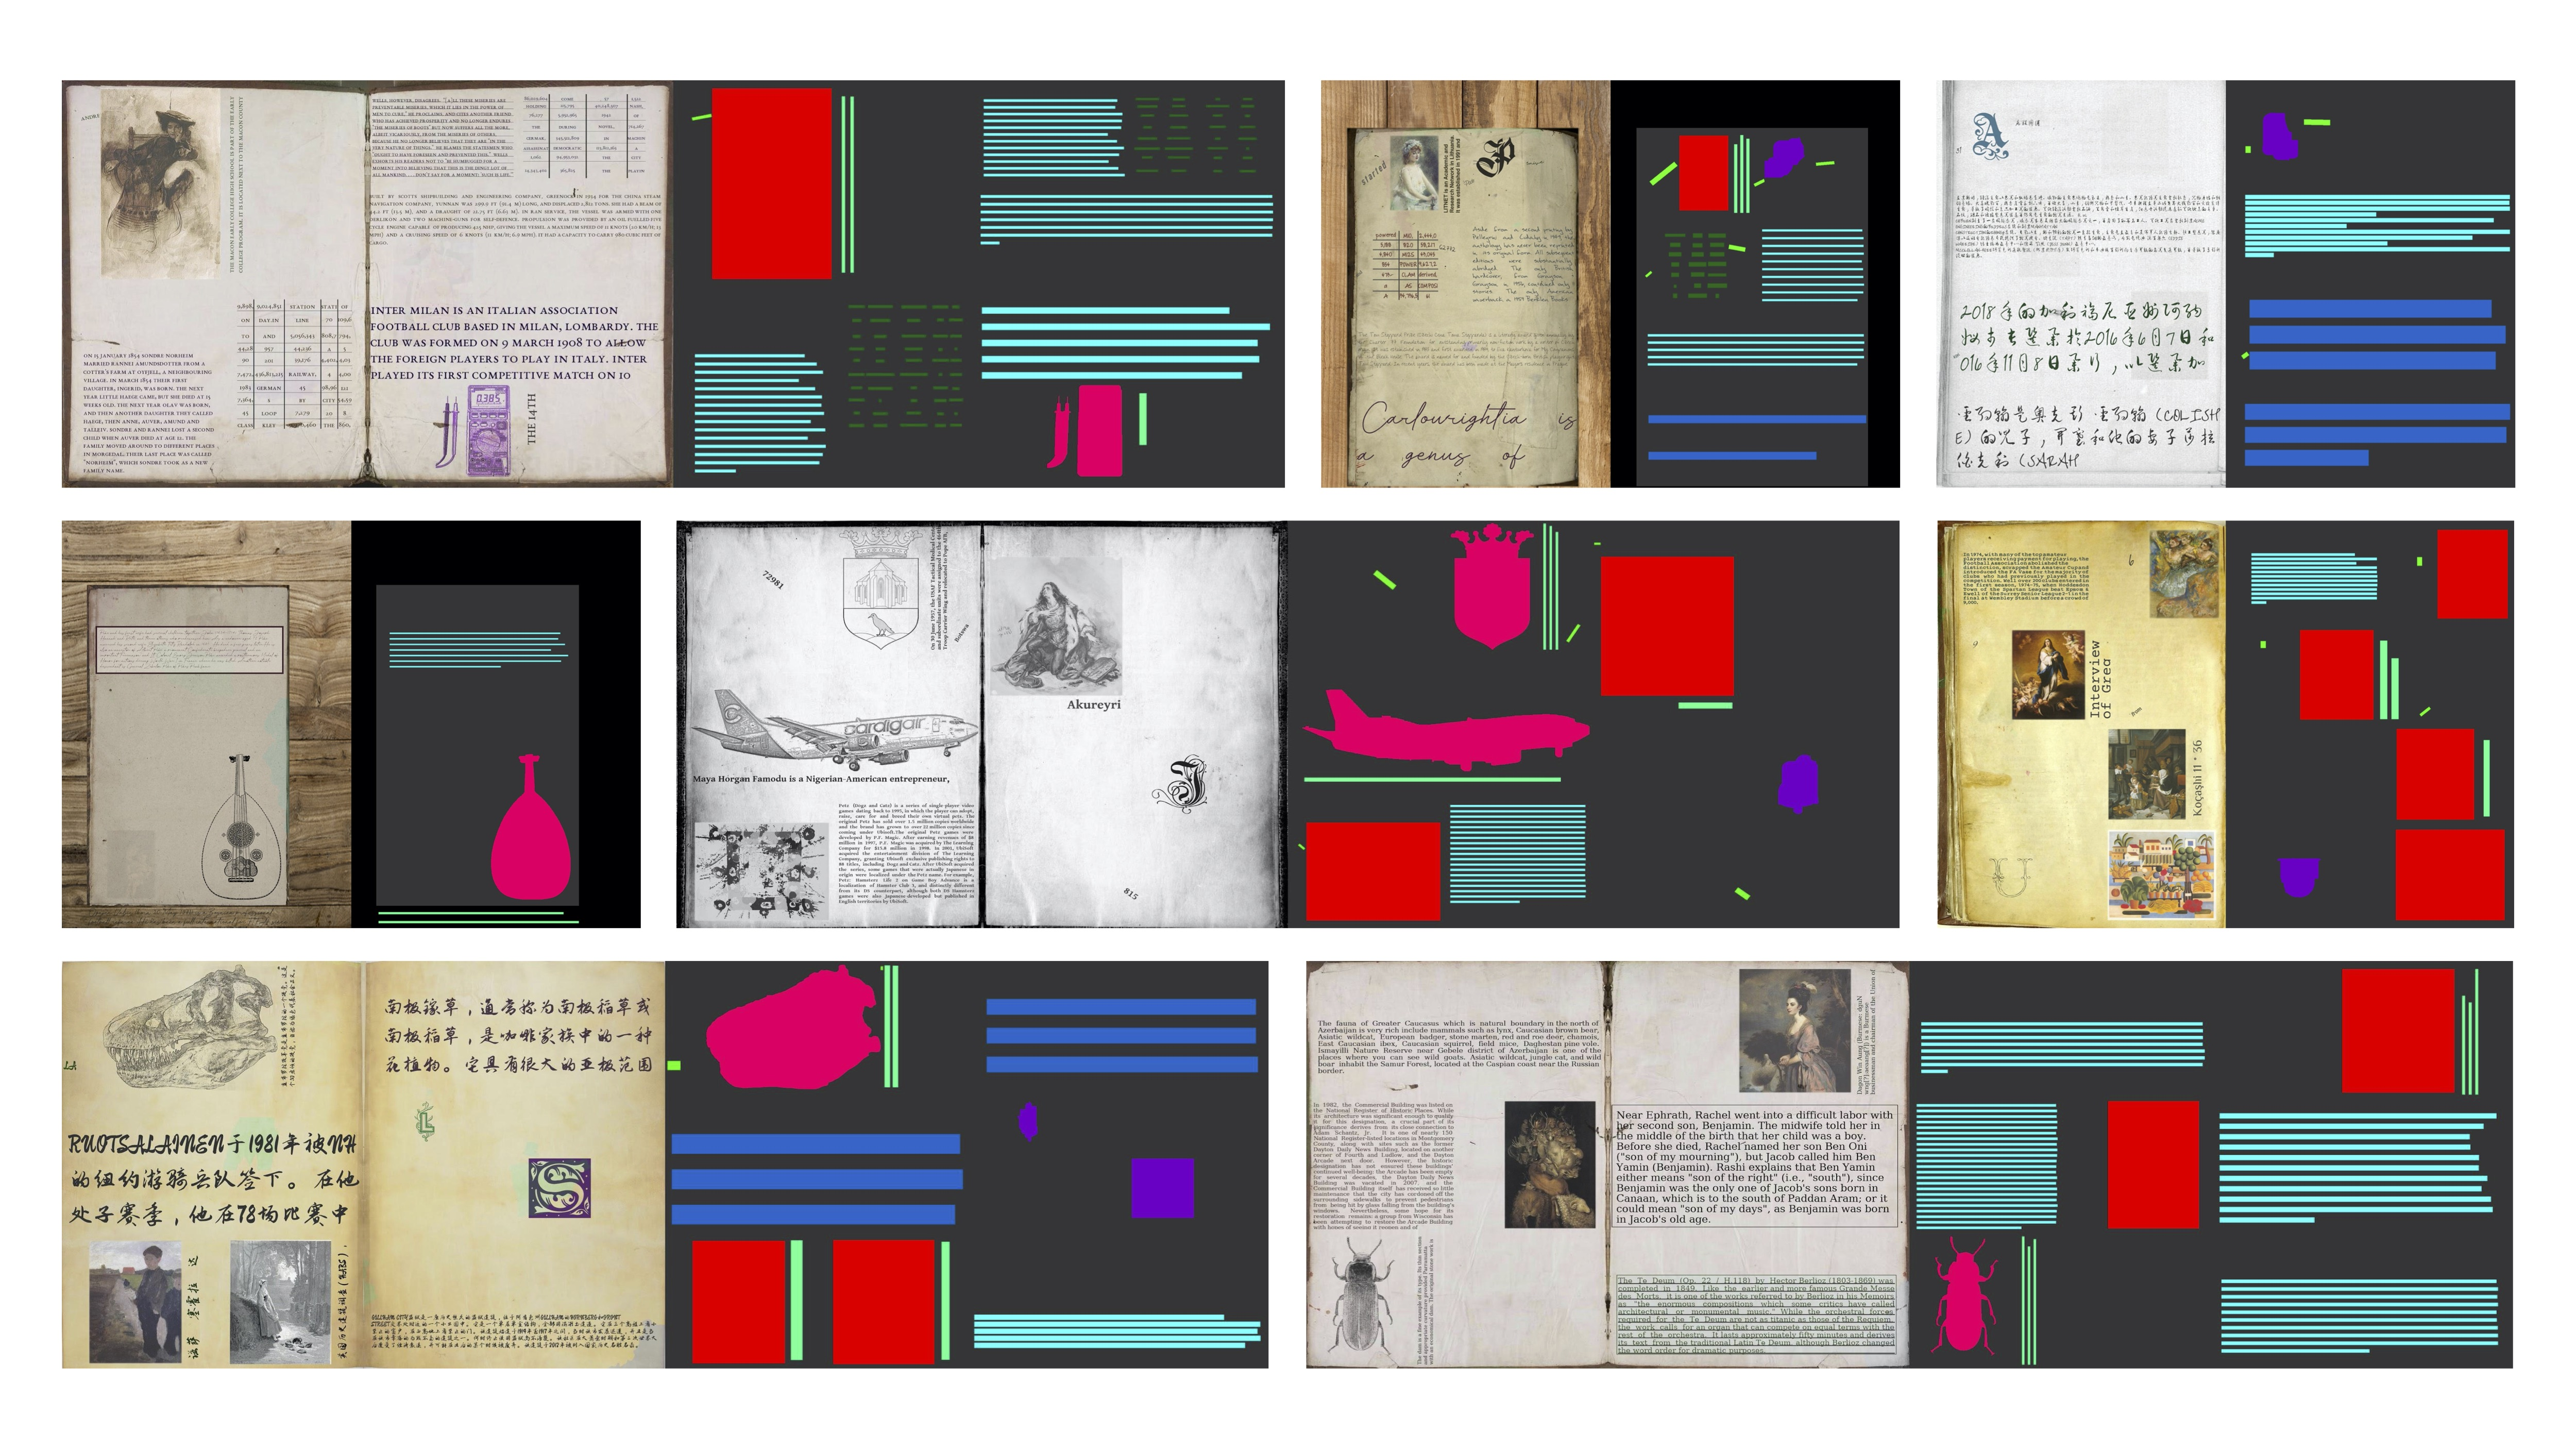
\includegraphics[width=13cm]{images/syndoc.jpg}
   		\caption{Exemples tirés d'un jeu de données généré avec SynDoc}
   		\label{fig:syndoc}
   	\end{figure}
   	
   	Contrairement à \yolov, \docex est donc développé spécifiquement pour le traitement des sources historiques, en prenant en compte les spécificités de ces documents iconographiques : le modèle est ainsi adapté au traitement d'images de pages contenant du texte et des illustrations, et prévoit également des outils de traitement du texte, tels que la détection des lignes en prévision\footnote{La détection des lignes est une étape préliminaire de traitements tels que la reconnaissance optique de caractères (OCR) ou la reconnaissance de l'écriture manuscrite (HTR).}. \docex semble ainsi être le modèle à favoriser dans le cadre des projets mentionnés dans ce mémoire, cependant, les premières évaluations des modèles\footnote{Les deux modèles ont fait l'objet d'un entraînement préliminaire sur des sources historiques qui ne sont cependant pas celles des deux projets, pour un premier affinement de leurs performances.} sur les sources d'\eida et de \vhs semblent témoigner de performances équivalentes.
   	
   	En effet, les détections de diagrammes lancées sur des sources du corpus \eida en prévision de leur annotation par les chercheurs pour la constitution du jeu d'entraînement ont témoigné de performances prometteuses aussi bien pour \docex que pour \yolov  (fig. \ref{fig:performances_modeles}), avec des diagrammes non-détectés dans les deux cas : les performances de chacun des deux modèles varient en fonction des pages, et il sera donc nécessaire de les départager en évaluant plus précisément leurs performances en amont de l'entraînement, puis après un premier entraînement des deux modèles sur les sources du projet\footnote{Sur le projet \eida, les modèles ont été fournis par les chercheurs du laboratoire \imagine et l'ingénieur du projet \vhs, n'ont donc pas encore été évalués sur les sources astronomiques du projet. La vérité de terrain étant encore en cours de production à l'été 2023, l'évaluation sera faite à partir d'un fragment de ce jeu de données lorsqu'il sera disponible.}. En tant que modèles \textit{off-the-shelf} en libre accès, \yolov et \docex ont pour vocation d'être efficaces et performants même sans entraînement sur des données spécifiques, et permettent ainsi de mener de manière satisfaisante des tâches de détection et d'extraction sur des données personnelles. Cependant, pour obtenir de meilleures performances, il est préférable d'entraîner ces modèles \textit{off-the-shelf} sur des images tirées du corpus du projet, pour l'adapter et le spécialiser dans la résolution de ces problèmes particuliers.
   	
\subsection{Entraînement et \textit{fine-tuning} d'un modèle de détection}
    \subsubsection{Démarche et volume des données}
	L'entraînement d'un modèle sur un jeu de données spécifiques permet de préciser les tâches effectuées et d'obtenir un modèle adapté aux besoins spécifiques de chaque projet. L'utilisation d'un modèle pré-entraîné permet, comme mentionné précédemment, de pallier aux limites de jeux de données avec trop peu d'exemples, en exploitant les représentations apprises précédemment et en les spécialisant sur les données spécifiques du projet qui l'utilise.
	
	\begin{figure}[H]
		\begin{subfigure}{1\linewidth}
			\centering
			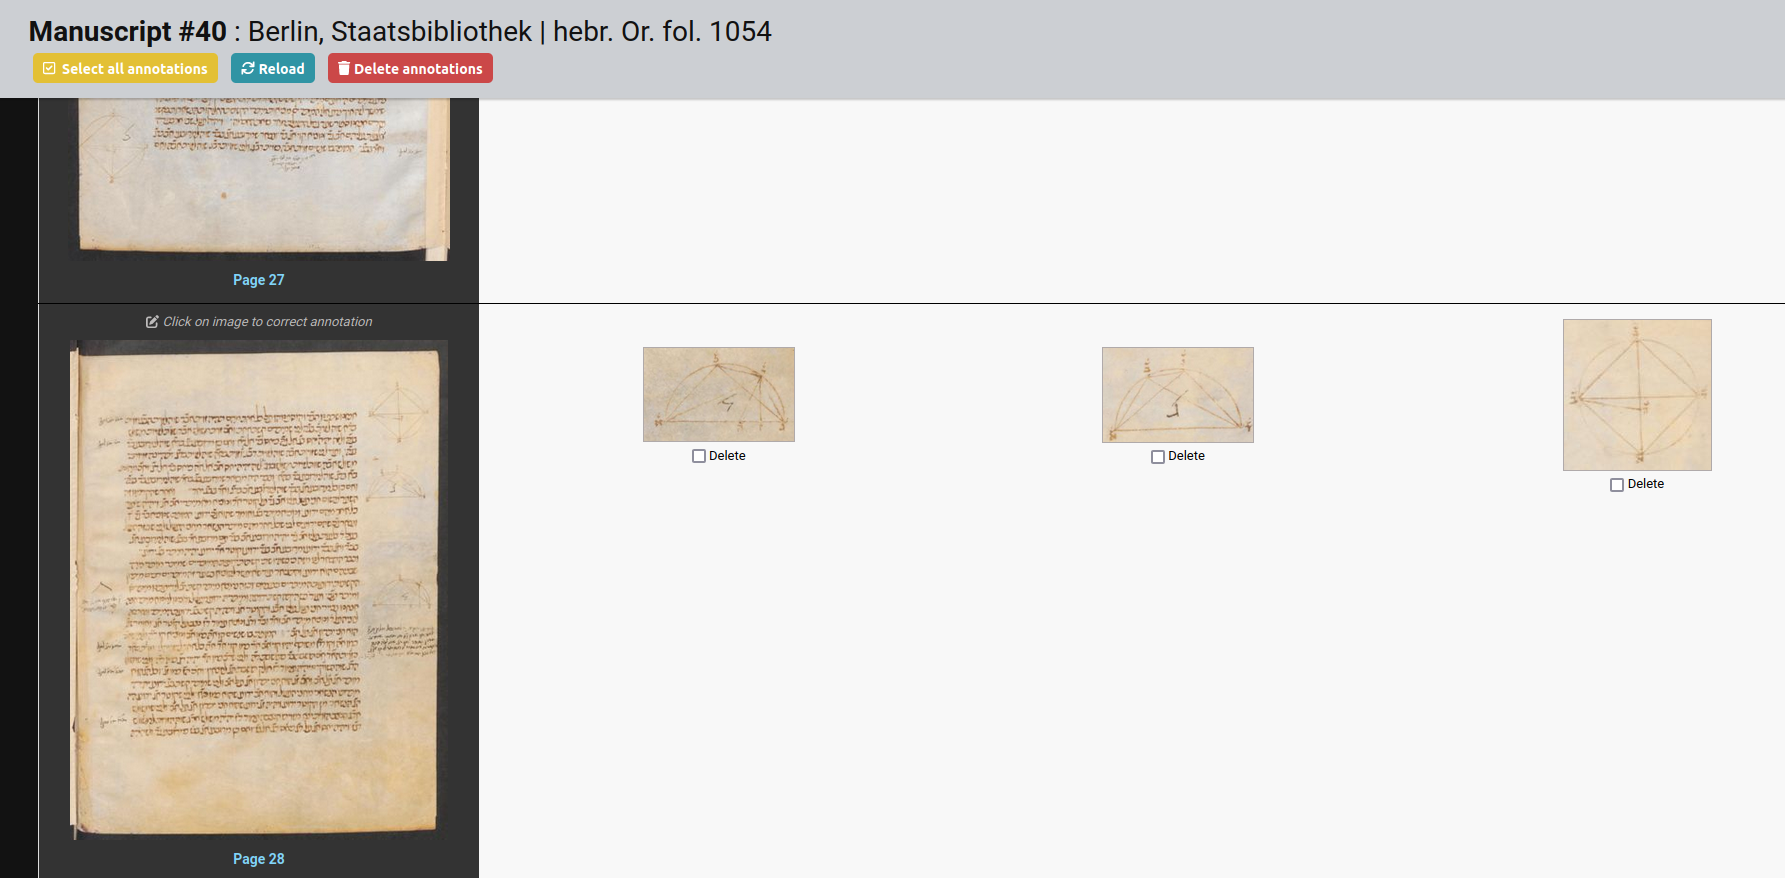
\includegraphics[width=10cm]{images/ms40_p28_docext.png}
			\subcaption{p. 28, \docex}
		\end{subfigure}
		\hspace{1pt}
		\begin{subfigure}{1\linewidth}
			\centering
			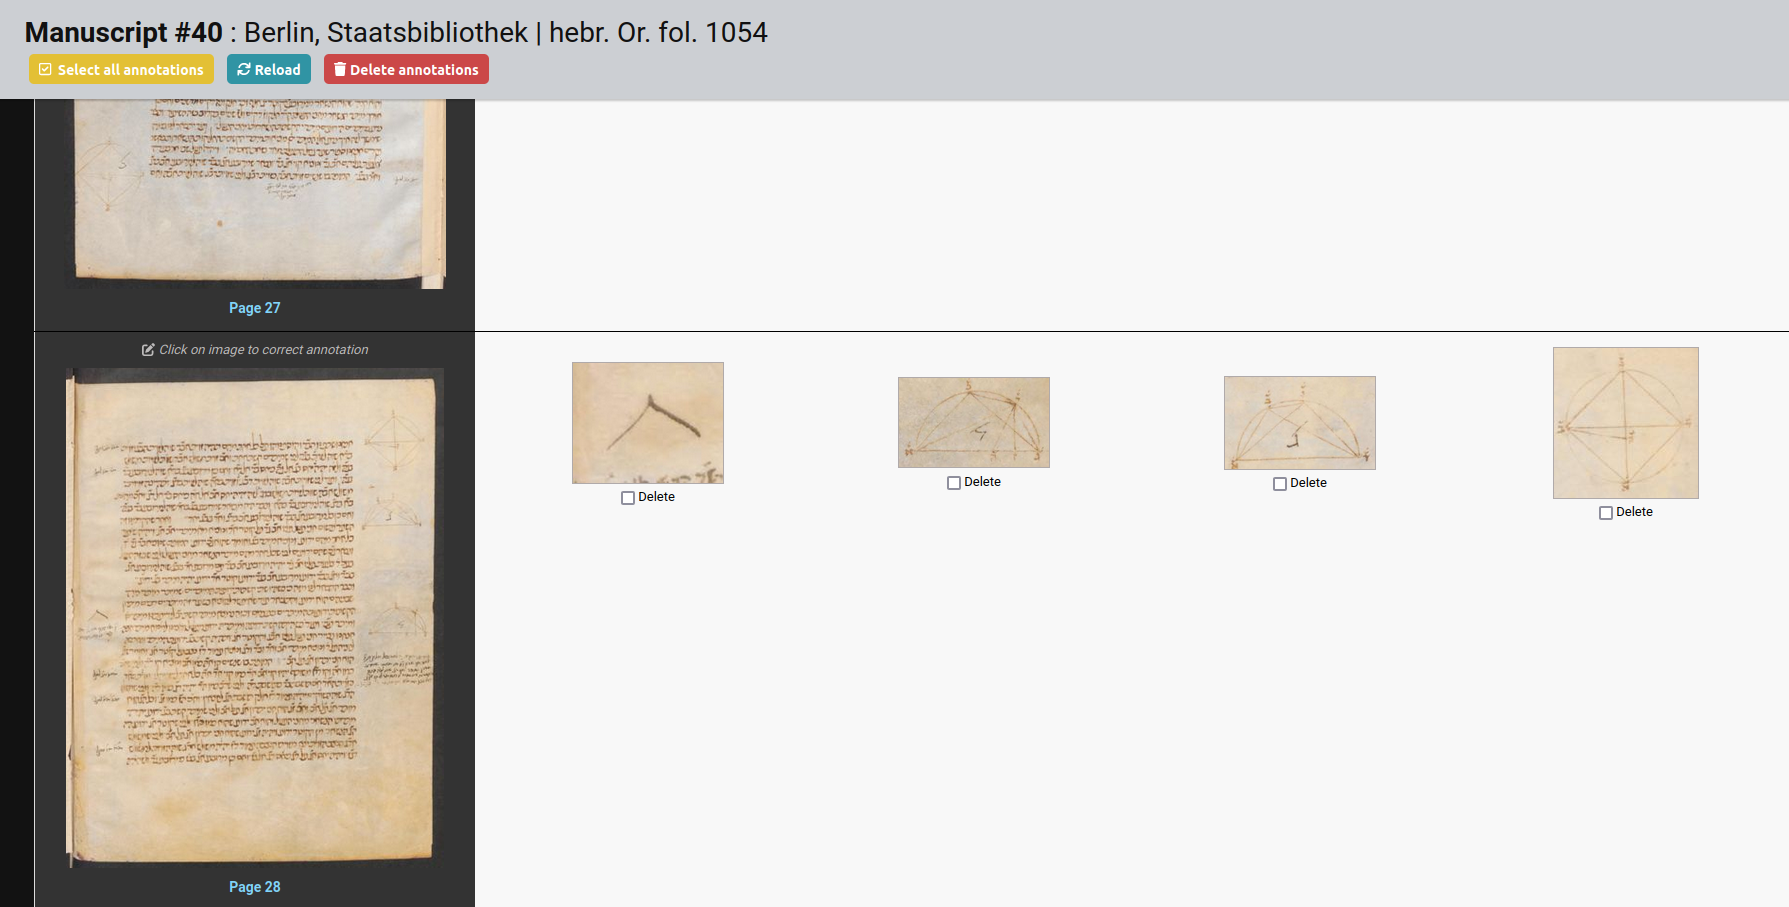
\includegraphics[width=10cm]{images/ms40_p28_yolov5.png}
			\subcaption{p. 28, \yolov}
		\end{subfigure}
		\begin{subfigure}{1\linewidth}
			\centering
			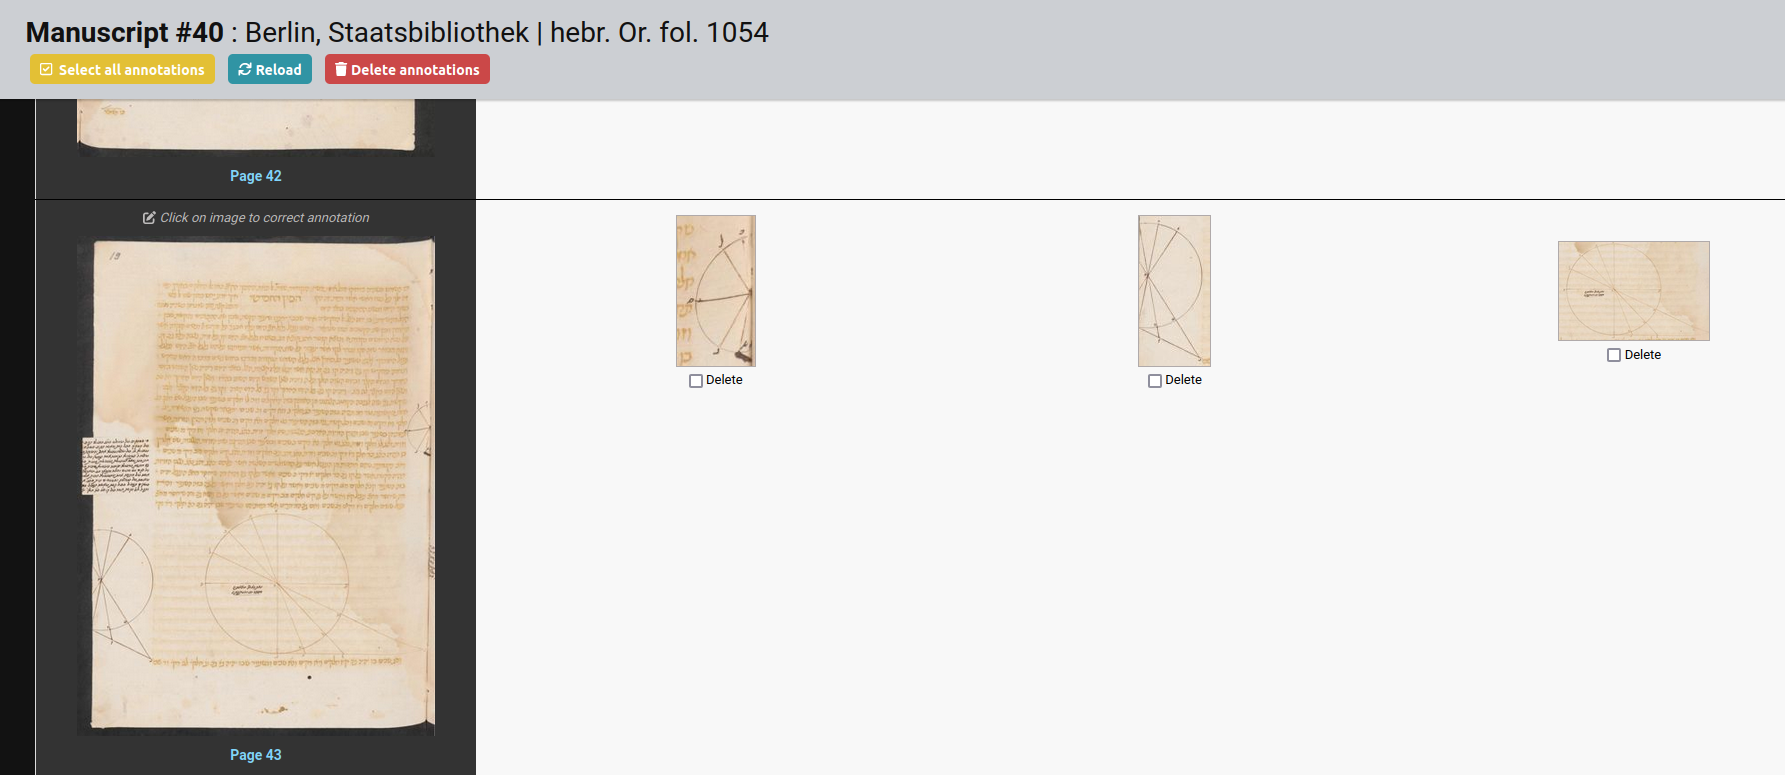
\includegraphics[width=10cm]{images/ms40_p45_docext.png}
			\subcaption{p. 45, \docex}
		\end{subfigure}
		\hspace{1pt}
		\begin{subfigure}{1\linewidth}
			\centering
			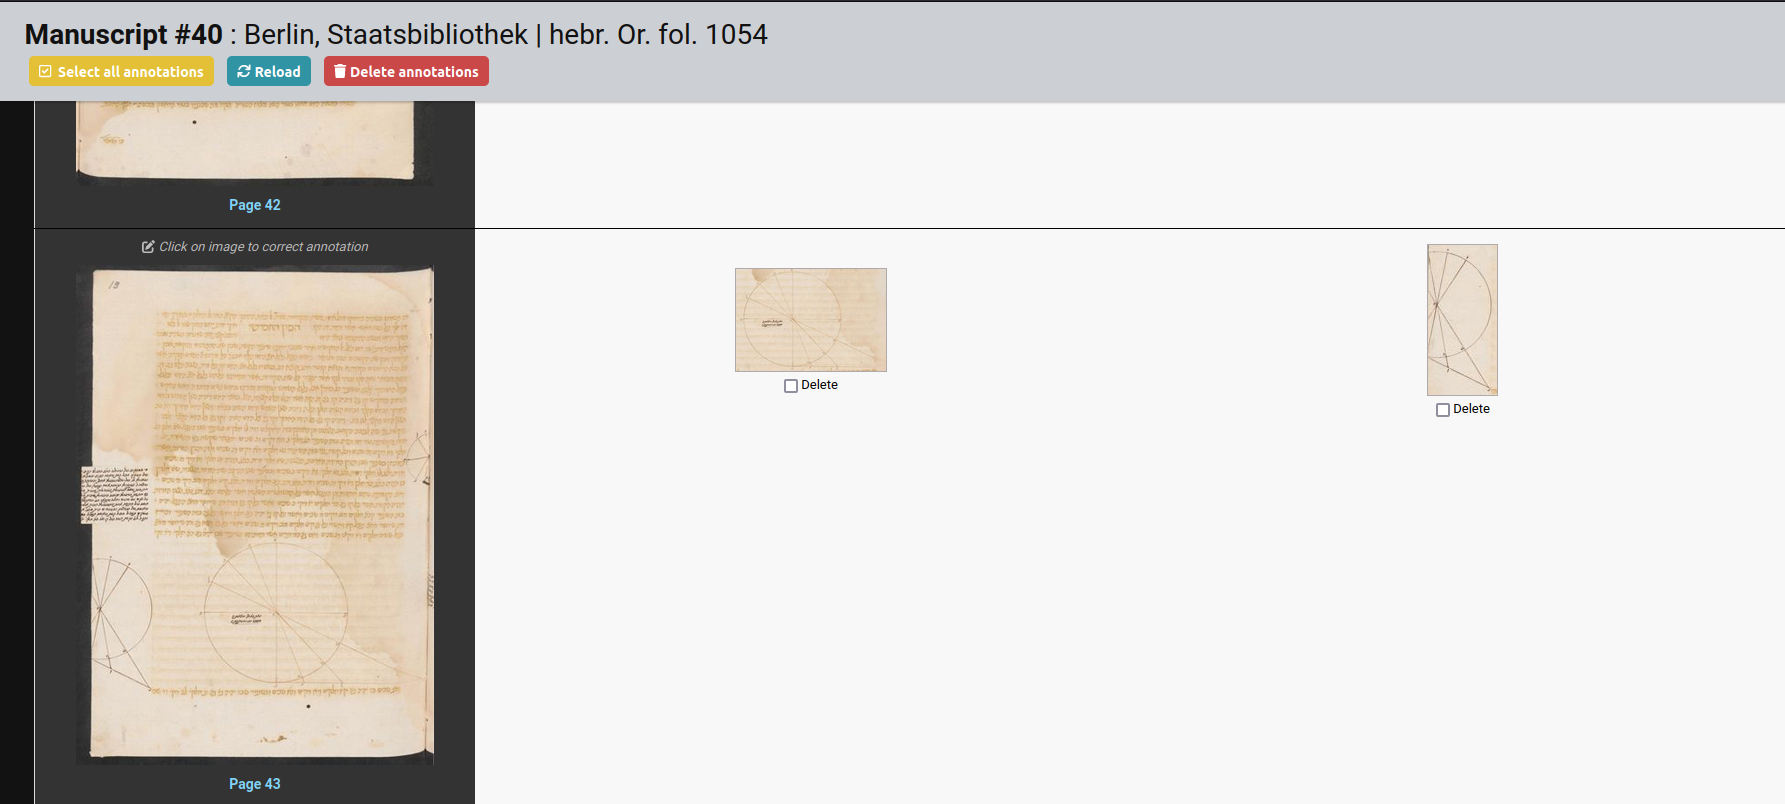
\includegraphics[width=10cm]{images/ms40_p45_yolov5.png}
			\subcaption{p. 45, \yolov}
		\end{subfigure}
		\caption{Diagrammes détectés par les modèles \yolov et \docex dans deux pages du manuscrit hebr. Or. fol. 1054 de la Staatsbibliotek (Berlin).}
		\label{fig:performances_modeles}
	\end{figure}

	Les modèles de détection \textit{off-the-shelf} comme \yolov prévoient souvent un \textit{workflow} pour l'entraînement du modèle\footcite{sharmaTrainingYOLOv5Object2022} par des projets qui souhaiteraient le spécialiser. Ainsi, dans le cas de \yolov, l'entraînement étant prévu par les développements mis à disposition par Ultralytics, il est nécessaire pour les ingénieurs de prévoir des jeux de données d'entraînement adaptés au format requis par le modèle\footnote{Les projets \vhs et \eida emploient tous deux \yolov comme modèle, ou \docex intégré au \textit{workflow} développé par Ultralytics pour \yolov : la structure des jeux de données d'entraînement est donc la même pour les deux modèles.} : l'annotation par les chercheurs doit donc être effectuée en prenant en compte ces restrictions, et les outils développés par les ingénieurs pour l'annotation des images doivent avoir pour sortie des fichiers aux formats appropriés. Un document de spécification sur les formats d'image et d'annotation a été réalisé dans le cadre du projet \eida (Annexe \ref{YOLOv5Training}), pour garder traces des besoins techniques de l'entraînement, étape suivante du projet. 
	
	L'entraînement d'un modèle \yolov se fait à partir d'un \textit{dataset} d'images et d'étiquettes (\textit{labels}) : il s'organise ainsi en un dossier de fichiers image (au format .png ou .jpg), et un dossier de fichiers texte (au format .txt) contenant une liste d'objets. Chaque fichier texte correspond à un ou plusieurs fichiers image -- plusieurs dans le cas de numérisation d'ouvrages, notamment, qui se composent d'un fichier d'annotations par ouvrage numérisé et non par image -- et listent les objets détectés dans l'image, à raison d'une ligne par objet. L'objet est caractérisé par ses dimensions (selon un rectangle qui l'encadre) et ses coordonnées sur l'image. Par exemple, le fragment de ficher d'annotation suivant correspond aux quatre objets détectés sur la page 6 du manuscrit 5 (Alm. 1) de la Gurukul Kangri Haridwar Collection (fig. \ref{fig:annotation_ms143}) :
	
	\begin{lstlisting}
		6 ms143_0006.jpg
		243 1852 464 549
		168 7 763 618
		440 951 1174 1130
		919 47 851 826\end{lstlisting}

   	\begin{figure}[H]
		\centering
		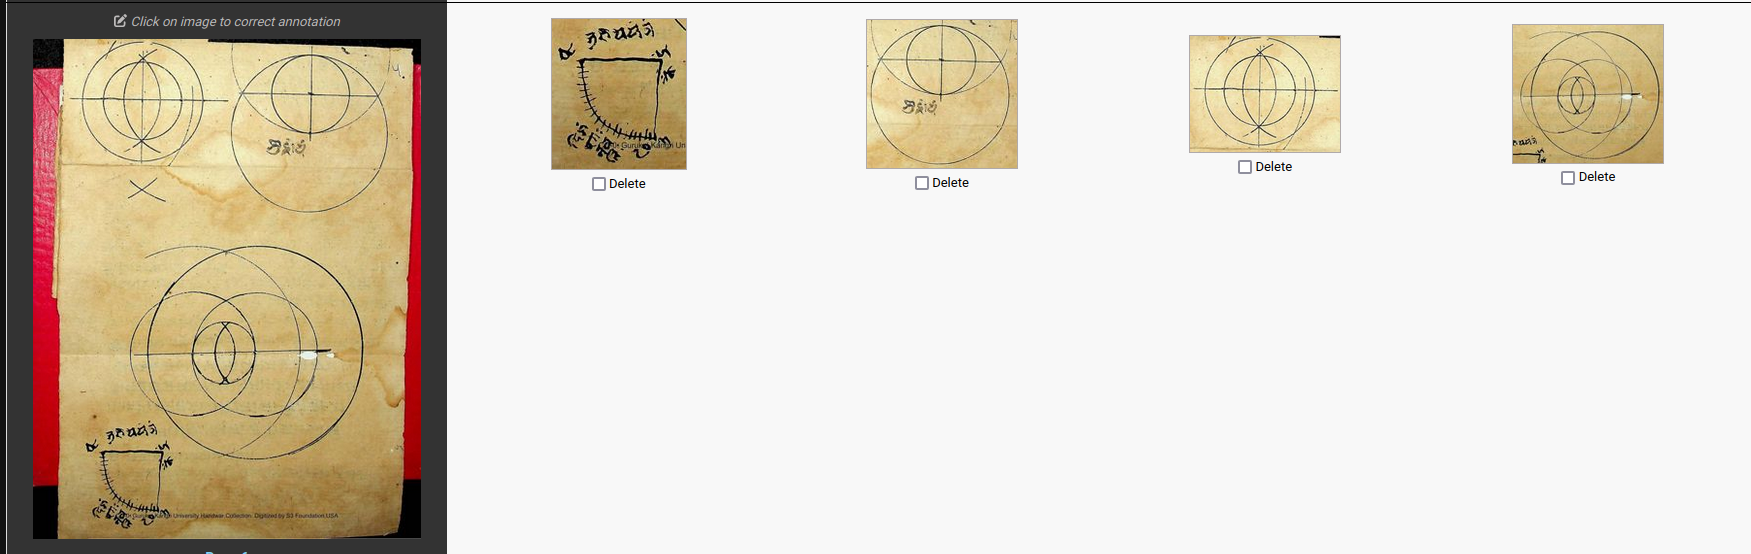
\includegraphics[width=15cm]{images/ms143_p6.png}
		\caption{Objets détectés sur la page 6 du manuscrit 5 (Alm. 1) de la Gurukul Kangri Haridwar Collection }
		\label{fig:annotation_ms143}
	\end{figure}

	À partir de cet ensemble d'images et d'annotations, l'entraînement peut être effectué : \yolov prévoit un script pour l'entraînement d'un modèle, dont seuls les paramètres doivent être modifiés pour l'adapter aux besoins du projet. Ainsi, les modèles de détection \textit{off-the-shelf} tels que \yolo ou \docex prévoient la possibilité d'un entraînement, simplifié par la mise à disposition d'outils permettant d'effectuer cette étape en écrivant peu de code. Cette volonté de rendre accessibles des outils adaptables, construits comme un socle solide pour des objectifs variés, permet l'intégration de la vision artificielle à des projets divers, sans demander de ces derniers de créer ou d'entraîner de zéro des réseaux de neurones ou des modèles de détections. La détection étant, en effet, une tâche de base de la vision par ordinateur, il est peu pertinent d'allouer des ressources pour reproduire des techniques déjà appliquées par de nombreux projets, et les outils \textit{off-the-shelf} offrent donc la liberté d'envisager la vision artificielle comme élément d'une chaîne de traitement des sources en allégeant les besoins et ressources -- notamment humains et temporels -- que demandent le développement et l'application de ces techniques. 

    \subsubsection{Sur-ajustement et diversité des exemples}
	L'utilisation d'un modèle pré-entraîné permet d'obtenir un modèle de détection fonctionnel malgré une faible quantité de données disponibles, puisque celui-ci a la capacité de généraliser les caractéristiques apprises à partir des données de pré-entraînement et de les appliquer aux données spécifiques du projet. Un trop faible volume de données présente en effet le risque de produire un modèle peu performant à cause du sur-ajustement (ou \textit{overfitting}) : on parle de sur-ajustement lorsqu'un modèle est bien ajusté aux données d'entraînement, mais incapable de généraliser face à de nouvelles données\footcite{cholletApprentissageProfondAvec2020a}. 
	
	Il est crucial de prévoir, lors de la constitution du jeu de données d'entraînement, une portion dédiée à la validation : on considère généralement que 20\% du jeu de données total est un volume suffisant pour cette étape. Les données de validation sont des données -- dans le cas de la détection, des images et annotations produites par des humains -- qui n'ont jamais été vues par le modèle et n'ont donc pas été utilisées pour l'entraînement. Comme les données d'entraînement, ces données de validation doivent être représentatives et diversifiées, puisqu'elles permettent de vérifier les performances du modèles, et d'identifier un sur-ajustement si le modèle ne donne pas, après entraînement, des résultats satisfaisants sur cet ensemble. Les données de validation permettent de mettre en avant les pertes à mesure que le modèle s'ajuste aux données d'entraînement\footcite{carremansHandlingOverfittingDeep2019}.
	
	Pour prévenir le sur-ajustement d'un modèle\footnote{Il existe diverses méthodes pour corriger le sur-ajustement d'un modèle de détection après entraînement, cependant, ce mémoire traitant de l'intégration de la vision artificielle à une chaîne de traitement des sources par le prisme du lien avec les équipes de recherche en histoire, nous n'aborderons pas ces questions qui concernent plus spécifiquement les aspects techniques de la création d'un modèle de détection. \cite{carremansHandlingOverfittingDeep2019}}, il est nécessaire de prévoir un jeu de données d'entraînement au volume suffisant -- supérieur à plusieurs milliers d'exemples dans le cas d'images\footnote{Le projet \eida compte plusieurs dizaines de milliers de pages dans son jeu de données d'entraînement.} -- et à la diversité représentative des données que le modèle pourra rencontrer. Le modèle de détection entraîné présente une capacité de généralisation qui rend son application pertinente pour le traitement des sources : l'entraînement d'un modèle \textit{off-the-shelf} permet ainsi de partir d'un modèle relativement performant dans des contextes variés et d'obtenir un modèle répondant aux besoins du projet, en trouvant l'équilibre entre manque d'ajustement et sur-ajustement.